\chapter{Il Gradiente di sottosterzo}
\label{cha:cap2}
Una classica caratteristica del comportamento in curva di un veicolo, è il concetto di
sottosterzo, sovrasterzo o sterzo neutro (introdotto nella sez.\ref{Dinamica laterale}).\\
Si può esprimere questo concetto (in modo semplice) basandosi sull’interazione tra la velocità di avanzamento e la 
curvatura durante la percorrenza di una curva in condizioni stazionarie:\\
Se all’aumentare della velocità del veicolo cresce la curvatura percorsa allora 
siamo in condizione di sottosterzo.
Quando la curvatura rimane invariata all’aumentare della velocità allora siamo in
condizione di sterzo neutro.\\
Per lo studio della stabilità direzionale dei veicoli era necessario avere un indicatore intuitivo che descrivesse le
differenze tra i casi elencati;\\ 
Il gradiente di sottosterzo è un parametro chiave utilizzato per quantificare e comprendere questo comportamento.\\
Questo concetto è stato introdotto per la prima volta da Olley nel 1946 \cite{Olley1946RoadMO}:\\
-Olley definì la "Linea di sterzo neutro" come il punto dove qualsiasi forza esterna applicata non produce alcun momento
d'imbardata addizionale durante una curva ed Il gradiente di sottosterzo sarà dunque la distanza longitudinale tra il 
centro di massa e la linea di sterzo neutro.
Sebbene non siano state ricavate espressioni matematiche questo concetto coinvolge le derivate degli angoli di deriva dei
pneumatici.\\
-A seguito dell'introduzione della sterzata cinematica (Ackermann), fù proposta un nuova formulazione definita come la differenza tra l'angolo di sterzo di riferimento e l'angolo di sterzo cinematico : $Ua_y = \delta_{REF} - \delta_A$ \cite{society1965vehicle}.\\
-Nel 1973 Pacjeka, studiò il concetto di gradiente di sottosterzo, scrivendo l'articolo \cite{doi:10.1080/00423117308968439}, nel quale presentava un metodo approssimato che permetteva di
creare un diagramma (handling diagram) utile per analizzare la stabilità in curva di un veicolo 
stradale in condizioni stazionarie.\\
Nella seconda parte dell'articolo \cite{doi:10.1080/00423117308968440} dimostrò, utilizzando il modello a singola traccia linearizzato ed esaminandone i poli, come il sottosterzo garantisca la stabilità in curva in condizioni stazionarie.\\
-Nel 1996 tramite lo standard SAE \cite{J266_201811}, si definirono le procedure per i test di controllo direzionale dei veicoli stradali, in modo da considerare le varie possibili condizioni di prova. \\
Furono apportate,inoltre, delle migliorie nella formulazione basata sulla sterzata cinematica, aggiungendo la possibilità di includere lo sterzo posteriore, in questo caso l'angolo di riferimento è dato dalla differenza tra l'angolo di sterzo anteriore e posteriore.\\
-Recentemente Guiggiani formulò delle perplessità riguardanti le definizioni del gradiente di sottosterzo esistenti, sostenendo che fossero chiaramente definite per veicoli a 4 o più ruote.\\
In un primo momento propose un miglioramento del $K_{SAE}$ per renderlo indipendente dal passo dei veicoli.
Successivamente propose un nuovo approccio all'handling che analizzeremo in seguito.
%-------------------------------------------------------------------------------------------------------
\section{Formulazioni classiche del gradiente di sottosterzo}
Le tre formulazioni maggiormente utilizzate sono: $K_{Pacejka}$ , $K_{SAE}$ , $K_{Guiggiani}$.
\subsection{Formulazione di Pacejka}
Pacejka introdusse il concetto di gradiente di sottosterzo per veicoli a trazione anteriore (FWD), inizialmente concentrando l'attenzione su modelli lineari e successivamente estendendolo a modelli non lineari.\\
Per pneumatici lineari, le forze sono definite come $F_{yf} = C_f \alpha_f$ e $F_{yr} = C_r \alpha_r$, 
La relazione tra l'angolo di sterzo anteriore, la curvatura e la velocità può essere scritta omettendo la derivata rispetto
al tempo:\\
\begin{equation} \label{7}
\frac{1}{R} = \frac{ C_f C_r l}{C_f C_r l^2 - mu^2(C_f a - C_rb)} \delta
\end{equation}

Combinando con $\rho = \frac{r}{v_x} = \frac{1}{R}$, si ottiene:
\begin{equation} \label{8}
\delta_f = \frac{1}{R} (l - mu^2\frac{C_f a - C_r b}{l C_f C_r})
\end{equation}
il Gradiente di sottosterzo è definito con $\eta$:
\begin{equation}
    K_{Pacejka} = \eta = -\frac{mg}{l} \frac{C_fa-C_rb}{C_fC_r} = -\frac{s}{l} \frac{mgC}{C_fC_r}
\end{equation}
\begin{figure}[!h]
    \centering
    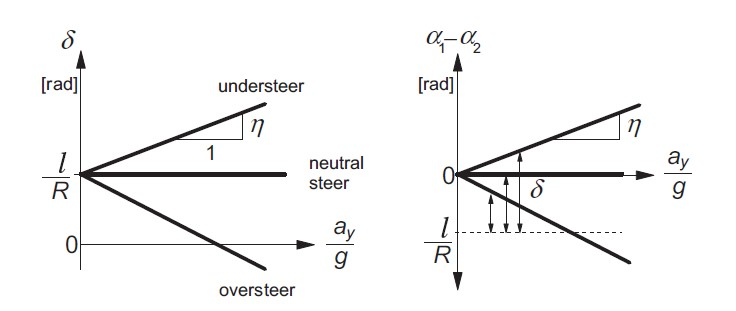
\includegraphics[scale=0.7]{Immagini/Understeer Gradient/Pacjeka understeer gradient.jpg}
    \label{fig:Pacjeka understeer gradient}
    \caption{Il gradiente di sottosterzo secondo la formulazione di Pacjeka}
\end{figure}
L'equazione \ref{7} scritta per il modello lineare può essere riscritta:\\
\begin{equation}
\delta_f = \frac{l}{R}( 1 + \eta\frac{u^2}{gl} ) = \frac{l}{R} + \eta \frac{a_y}{g}
\end{equation}
In condizioni non lineari, il gradiente di sottosterzo deriva dalla geometria (sterzata cinematica, Ackermann):\\
\begin{equation}
\frac{d\delta_f}{da_y} = \frac{d(\alpha_f - \alpha_r)}{da_y}
\end{equation}
Si può ricondurre la formulazione al $K_0$:
\begin{equation}
K_{Pacejka} = \frac{d(\alpha_f - \alpha_r)}{d(a_y/g)} = -\frac{g}{l} K_0
\end{equation}

\subsubsection{Handling Diagram}
Per migliorare la comprensione del comportamento direzionale in condizioni non lineari, Pacjeka nel suo libro
\cite{pacejka2005tire} introdusse un metodo grafico per visualizzare intuitivamente la risposta del veicolo.
Tale metodo è basato sugli angoli di deriva dei pneumatici.

\subsection{Formulazione SAE}

La formulazione SAE è anch'essa basata sulla geometria della sterzata di Ackermann, considera veicoli a 4 ruote sterzanti,
definendo:\\
Angolo di sterzo di Ackermann (cinematico) come $\delta_A = \frac{L}{R}$.\\ 
Angolo di sterzo di riferimento come $\delta_{\text{ref}} = -\delta_f + \delta_r$.\\
Il gradiente di sottosterzo è infine definito come la differenza tra loro derivate:
\begin{figure}[!h]
    \centering
    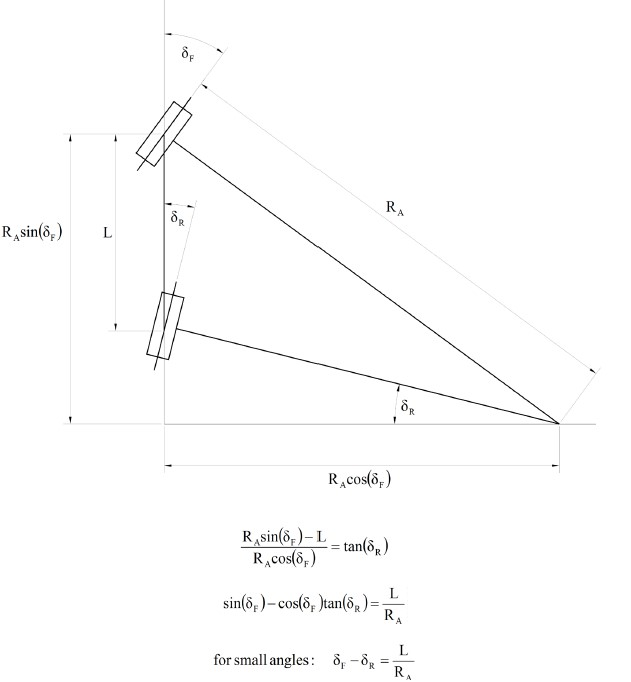
\includegraphics[scale=0.7]{Immagini/Understeer Gradient/Ackermann geometry.jpg}
    \caption{Angolo di sterzo cinematico}
    \label{fig:Delta ref}
\end{figure}
\begin{equation}
K_{SAE} = \frac{d\delta_{ref}}{da_y} - \frac{d\delta_A}{da_y} = \frac{d(-\alpha_f + \alpha_r)}{da_y}
\end{equation}
Potrebbe essere riportato al $K_0$ come segue:
\begin{equation}
K_{SAE} = l \cdot \frac{\partial \rho}{\partial a_y} = l \cdot K_0
\end{equation}



\subsection{Formulazione di Guiggiani}
Nel primo libro \cite{guiggiani2007dinamica} propose una formulazione in accordo con la definizione SAE \cite{J266_201811}:\\
\begin{equation}
    K_{\gamma} = \frac{d}{d\Tilde{a}_y} (\delta - \frac{l}{R}) = \frac{d}{d\Tilde{a}_y} (\alpha_{1p} - \alpha_{2p}) = \frac{d}{d\Tilde{a}_y} (\gamma_0 - \gamma_p)
\end{equation}
Che nel caso del modello lineare diventava:\\
\begin{equation}
    K_{\gamma} = \frac{m}{l}( \frac{\Phi_2 a_2 - \Phi_1 a_1}{\Phi_1 \Phi_2})
\end{equation}
Nella seconda edizione \cite{guiggiani2018science} criticò aspramente la definizione SAE come vedremo successivamente,
proponendo una nuova versione che migliorasse la precedente, che è funzione di due variabili:\\
\begin{equation} \label{roy 1}
    \rho_y = \rho_y(\delta_{va},\Tilde{a}_y)
\end{equation}
eccetto nel caso del modello a singola traccia con differenziale aperto,\\
allora $\rho_y = \rho_y (\Tilde{a}_y) = - df_{\rho}/d\Tilde{a}_y $ :
\begin{equation} \label{6.171}
    \rho_y = \frac{\partial \rho_p}{\partial \tilde{a}_y} = \frac{\partial}{\partial \tilde{a}_y} (\frac{1}{R}) = -\frac{K}{l}
\end{equation}
Questa è molto simile alla definizione classica del K ma con delle differenze sostanziali:\\
\'E definito per qualsiasi in quanto non è influenzato dal passo $l$ dei veicoli e neanche dallo sterzo di Ackermann.\\
Naturalmente, la derivata parziale nell'eq.\ref{6.171} richiede che l'angolo di sterzo sia mantenuto costante.
Nel caso di un test ad angolo volante fissato l'eq.\ref{6.171} può essere riscritta come:\\
\begin{equation}
    \frac{d\rho_p}{d\tilde{a}_y} = \frac{d(r_p/u_a)}{d(r_pu_a)} = \frac{d(r_p/u_a)}{du_a} (\frac{d(r_pu_a)}{du_a})^{-1} = \frac{1}{u_a^2} (\frac{\dot r_pu_a - r_p}{\dot r_pu_a + r_p}) = \rho_y
\end{equation}


\subsection{Confronto e limiti delle formulazioni classiche}

\subsubsection{Confronto}
Le tre formulazioni analizzate sono sostanzialmente equivalenti a $K_0$, condividendo la derivata 
dell'accelerazione laterale al denominatore.\\
\begin{figure}[!h]
    \centering
    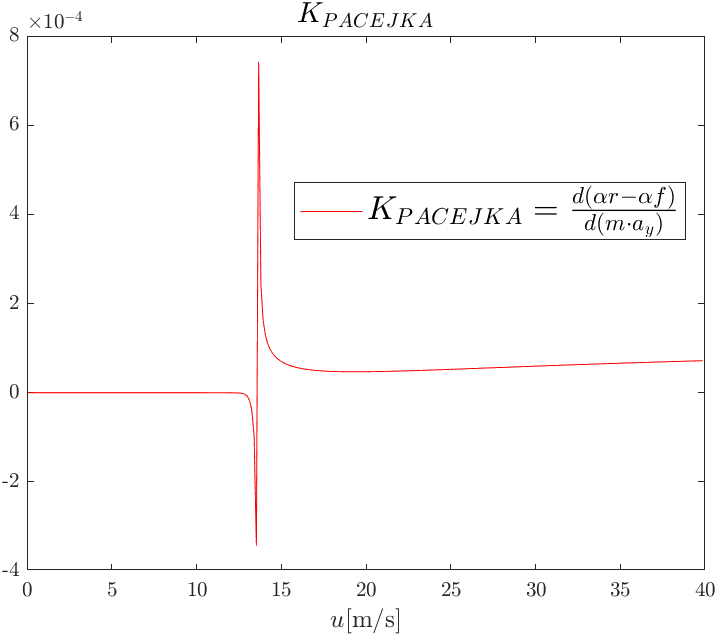
\includegraphics[scale=0.5]{Immagini/Understeer Gradient/Kpacejka.png}
    \caption{}
    \label{fig:Kpacejka}
\end{figure}
\begin{figure}[!h]
    \centering
    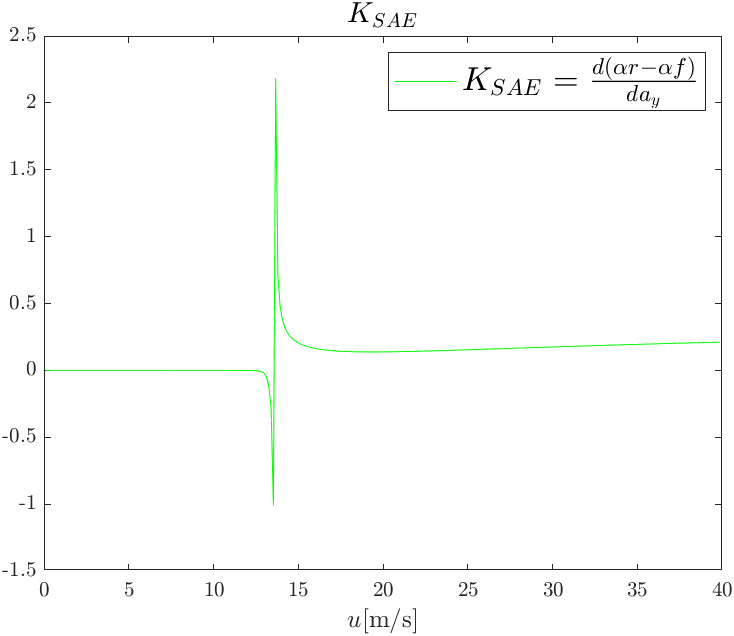
\includegraphics[scale=0.5]{Immagini/Understeer Gradient/Ksae.png}
    \caption{}
    \label{fig:Ksae}
\end{figure}
\begin{figure}[!h]
    \centering
    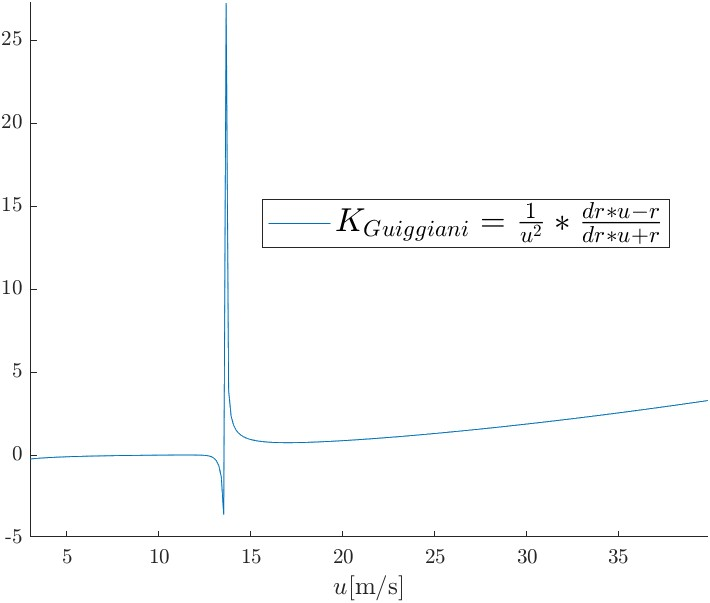
\includegraphics[scale=0.25]{Immagini/Understeer Gradient/Kguiggiani.jpg}
    \caption{}
    \label{fig:Kguiggiani}
\end{figure}

\subsubsection{Limiti}
Tutte e tre le formulazioni classiche condividono la derivata dell'accelerazione laterale al denominatore, 
questo genera una scarsa definizione nei punti di flesso.\\
Se si considerano angoli di sterzo costanti su entrambi gli assi, la derivata parziale può essere sostituita dal 
differenziale dunque $\frac{\partial \rho}{\partial a_y} \longrightarrow{} \frac{d \rho}{da_y}$. Essendo in condizioni
stazionarie, abbiamo $\rho = \frac{r}{u}$ e $a_y = r \cdot u$. Quindi, $K_0$ diventa:
\begin{equation}
K_0 = 
\frac{d \rho}{da_y} = \frac{d \left( \frac{r}{u} \right)}{d(ru)} = \frac{\frac{d(\frac{r}{u})}{du}}{\frac{dru}{du}} =
\frac{\frac{dr}{du} - \frac{r}{u}}{u^2( \frac{dr}{du} + \frac{r}{u})} =
\frac{\frac{d \rho}{du}}{u( \frac{dr}{du} + \frac{r}{u})}
\end{equation}
Il suo numeratore rappresenta esattamente il concetto di gradiente di sottosterzo, il cui segno indica la tendenza
sottosterzante, sovrasterzante o neutro.
$K_0$ descrive correttamente questa caratteristica finchè il segno del denominatore è costante. \\
Tuttavia, non è sempre costante:\\
A bassa velocità, la velocità d'imbardata ($r$) aumenta all'aumentare dell'accelerazione, $\frac{dr}{dv}$ risulta
positivo, essendo il denominatore positivo. \\
Man mano che la velocità d'imbardata si avvicina al suo limite massimo correlato al limite di accelerazione laterale,
questa inizia a diminuire, $\frac{dr}{du}$ diventa negativo (fig.\ref{fig:r vs u delta=0.145}).\\ 
Di conseguenza, il denominatore potrebbe diventare zero o negativo. Questo cambiamento nel segno del denominatore
interrompe la connessione tra $K_0$ e la caratteristica di sottosterzo. Inoltre, un denominatore intorno a zero causerebbe
instabilità numerica (fig.\ref{fig:K0 delta=0.145}).\\
\begin{figure}[!h]
    \centering
    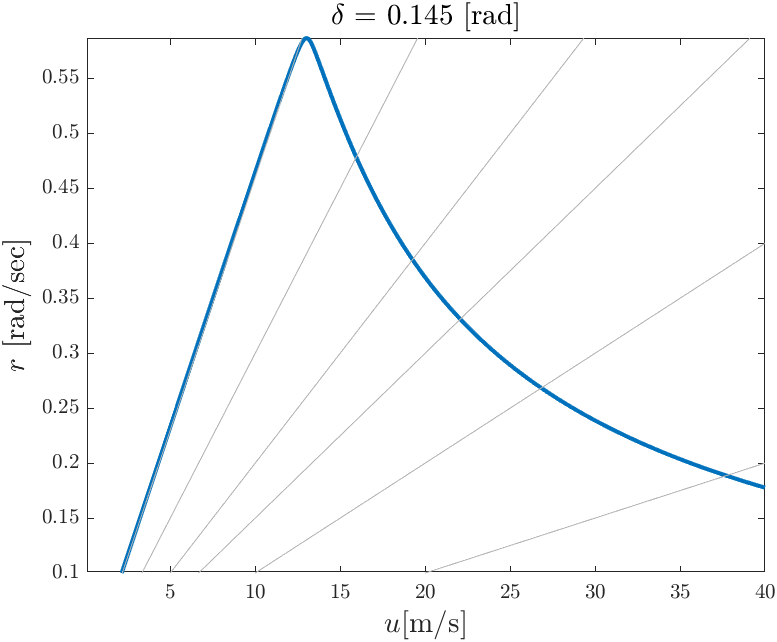
\includegraphics[scale=0.7]{Immagini/Understeer Gradient/r vs u.png}
    \caption{velocità d'imbardata e velocità}
    \label{fig:r vs u delta=0.145}
\end{figure}
\begin{figure}[!h]
    \centering
    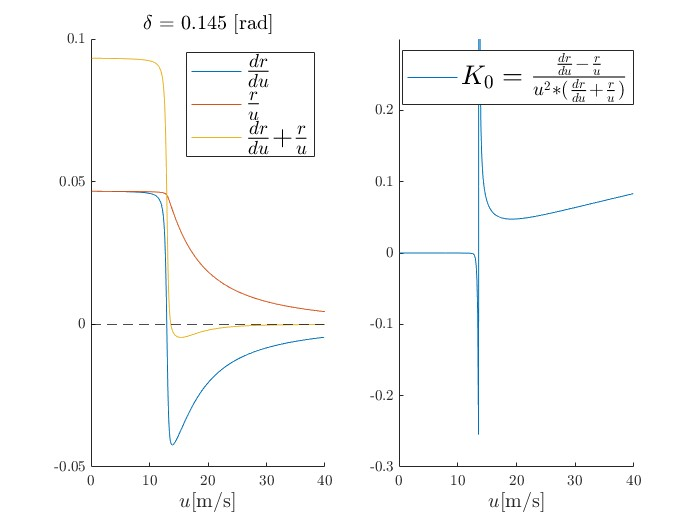
\includegraphics[scale=0.5]{Immagini/Understeer Gradient/K0.jpg}
    \caption{$K_0$}
    \label{fig:K0 delta=0.145}
\end{figure}
L'esempio mostrato nelle fig.\ref{fig:r vs u delta=0.145} e \ref{fig:K0 delta=0.145} rappresenta la velocità d'imbardata in
regime stazionario di un veicolo a trazione anteriore e pneumatici non lineari (rimandare ad appendice dove si spiega il
modello) che esegue una manovra ad angolo di sterzo fissato $\delta_f = 0.145$ e velocità crescente da 0 a 40 [m/s].\\
In particolare la fig.\ref{fig:r vs u delta=0.145} rappresenta la velocità d'imbardata al variare della velocità di avanzamento e le linee grigie rappresentano la curvatura.
La curvatura diminuisce per velocità superiori a 15 [m/s], indicando sottosterzo.\\ 
Il denominatore presenta il termine $\frac{dr}{du} + \frac{r}{u}$, quando $u$ è bassa, sono quasi costanti, indicando
sterzo neutro. Man mano che $u$ aumenta, $r$ arriva alla saturazione, causando una diminuzione di entrambi (sottosterzo).\\
In condizioni di saturazione $\frac{dr}{du}$ cambia di segno portando ad un cambio di segno nel denominatore.\\
La Fig. \ref{fig:K0 delta=0.145} rappresenta come il $K_0$ presenti un punto di singolarità quando il suò denominatore è 
prossimo allo zero.\\ 

\subsubsection{Definizione nei punti di flesso}
La fig.\ref{fig:Sterzo Dinamico} mostra come un veicolo stradale a tendenza sottosterzante con pneumatici non lineari 
presenti un punto di flesso nel diagramma dell'angolo di sottosterzo, il punto di flesso si verifica nel momento in cui i 
pneumatici anteriori raggiungono il picco di forza laterale che sono in grado di fornire ($F_y^{max} = \mu \cdot F_z$).
All'aumentare della richiesta d'accelerazione laterale i pneumatici non sono più i grado di generare le forze richieste
anzi oltre il picco la forza che riescono a generare è ancora minore.
La curvatura $\rho$ continua a diminuire (Raggio di curvatura $R = \frac{1}{\rho}$ continua ad aumentare).\\
\begin{figure}[!h]
    \centering
    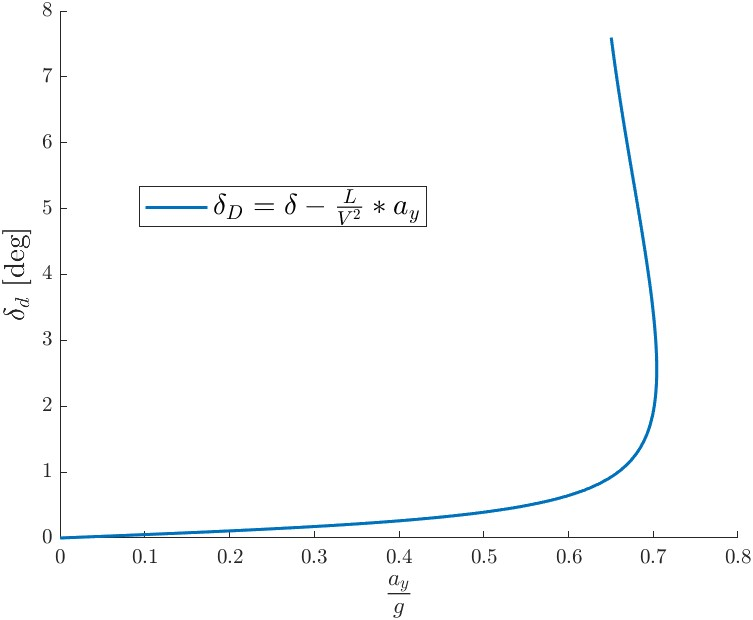
\includegraphics[scale=0.4]{Immagini/Understeer Gradient/Sterzo dinamico cinesi.jpg}
    \caption{}
    \label{fig:Sterzo Dinamico}
\end{figure}
$d\rho/da_y$ cambia il suo segno oltre il punto di flesso della curva:
Questo genera un ambiguità teorica per quanto riguarda la definizione di comportamento sovrasterzante o sottosterzante:\\
Nonostante sia chiaro il fatto che il veicolo nella pratica sia in completo scorrimento dell'assale anteriore
(completo sottosterzo), qualche ricercatore potrebbe esprimere dubbi sul fatto che oltre il punto di flesso riducendo
l'angolo di sterzo il veicolo riprenda direzionalità ($R$ diminuisce come nel caso di sovrasterzo).

\subsubsection{Critica di Guiggiani}
Il calcolo di $K$ necessita sia dell'angolo di sterzata $\delta_{ref}$ sia dell'angolo di sterzata di
Ackermann $\frac{l}{R}$.\\ 
Purtroppo, nessuno dei due è chiaramente definito in un veicolo reale. Infatti, sono ben definiti solo nel modello a
singola traccia. In un veicolo reale, le due ruote anteriori hanno tipicamente angoli di sterzata differenti risulta quindi
difficile definire con precisione l'angolo di sterzata $\delta_{ref}$.
Anche l'angolo di sterzata di Ackermann $\frac{l}{R}$ incontra difficoltà quando un veicolo ha tre o più assi, poiché il
passo $l$ non è più definito chiaramente. Nonostante la maggior parte delle auto dispongono di solo due assi non è corretto basare una teoria su un concetto così debole.\\


%-----------------------------------------------------------------------------------------------------------
\section{Formulazioni alternative del gradiente di sottosterzo}
\subsubsection{Una nuova formulazione del gradiente di sottosterzo basata sulla velocità}
In questo sotto paragrafo si vuole descrivere ed analizzare una nuova formulazione proposta in un articolo di ricerca in fase di revisione.
L'articolo in questione è stato creato dagli autori He Zhen, Guan Yihang ,Zhou Hongliang del "Harbin institute of technology, School of Astronautics" e da Miao Weiwei, Yu zhen del "Chassis Department FAW Group corporation".
il titolo "A new formulation of the understeer gradient and stability
margin to analyze vehicle steady-state cornering behaviour".\\

In questo articolo si propone una nuova formulazione che non sia dipendente dall'accelerazione laterale in modo da evitare
di incorrere nei problemi osservati precedentemente.
Questa nuova formulazione si propone per essere utilizzata in condizioni critiche (saturazione dei pneumatici) ed è
definita dalla derivata della curvatura rispetto alla velocità:  $K = \frac{\partial \rho}{\partial u}$ o $K = \frac{d \rho}
{du}$\\ %con l'ipotesi di angoli di sterzo costanti.\\
Può essere espressa in funzione della velocità di imbardata:
\begin{equation} \label{Kcinesi}
K = \frac{d \rho}{du} = \frac{d(ru)}{du} = \frac{dr}{du} - \frac{ru}{u}
\end{equation}

\begin{figure}[!h]
    \centering
    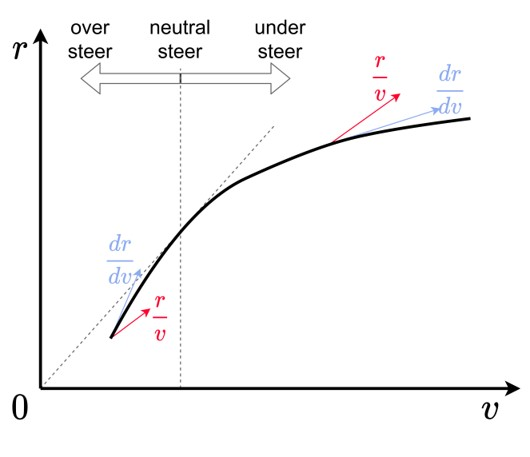
\includegraphics[scale=0.6]{Immagini/Understeer Gradient/K_cinesi.jpg}
    \caption{}
    \label{fig:K_cinesi}
\end{figure}
Questa formulazione funziona in modo simile alle formulazioni precedenti. 
$K$ positivo indica sovrasterzo, $K$ negativo indica sottosterzo e $K=0$ indica sterzo neutro.\\ 
Il segno di $K$ è determinato dal numeratore, che è la differenza tra la pendenza tangente $\frac{dr}{du}$ e la pendenza assoluta $\frac{r}{u}$ in ogni punto della curva $r$  $u$.\\ 
Questa differenza può essere ottenuta intuitivamente dalla curva stessa. La Fig.\ref{fig:K_cinesi} mostra che:\\ 
-Quando $\frac{dr}{du} > \frac{ru}{u}$ e $K > 0$, la curvatura aumenta, indicando sovrasterzo.\\ 
-Quando $\frac{dr}{du} < \frac{ru}{u}$ e $K < 0$, la curvatura diminuisce, indicando sottosterzo.\\
\'E sostanzialmente funzione di $r$ e $u$ e non coinvolge concetti complessi, questo la rende applicabile a diversi tipi
di veicoli, veicoli a sterzata anteriore tradizionale, veicoli a quattro ruote sterzanti, veicoli a quattro ruote
indipendenti e persino veicoli con più di quattro ruote.\\ 
\'E applicabile a prove di "rampspeed" cioè con angolo di sterzo fissato e velocità crescente mentre non è applicabile a
prove di "rampsteer".
Questo rappresenta un difetto di questa nuova formulazione.\\
Inoltre eliminando la dipendenza dall'accelerazione laterale si perde il nesso con la stabilità del veicolo del quale
abbiamo parlato nel cap.\ref{cha:cap1}, per risolvere questo inconveniente gli autori propongono l'aggiunta di un margine di stabilità, tuttavia questo è pur sempre un limite di questa formulazione.


\subsubsection{Bucchi e Frendo}

Le formulazioni classiche concentrano l'attenzione sul controllo dell'imbardata del veicolo utilizzando modelli fortemente semplificati sia per i pneumatici che per la dinamica del veicolo.\\
La nuova formulazione proposta nell'articolo \cite{doi:10.1080/00423114.2016.1167225} mette in relazione  il gradiente di sottosterzo alla coppia d'imbardata, a partire da manovre quasi stazionarie facilmente eseguibili su veicoli reali.\\
Questa formulazione si basa sulla conoscenza della derivata (rispetto al tempo) della curvatura e del momento d'imbardata generato dalle forze dei pneumatici.\\

(Partiamo dalle mappe di Guiggiani)
Poiché è dispendioso ottenere le mappe per tutte le combinazioni di $\Tilde{a_y}$ e $\delta_W$, si considerano manovre a velocità costante ($\dot{u} = 0$) e ($\dot{\delta_W} =$ costante) per ottenere informazioni sul comportamento dinamico del veicolo considerato. Queste manovre possono essere considerate rappresentative (con buona approssimazione ) delle comuni azioni di guida.\\
A partire dalla mappa $\rho_p(\Tilde{a_y}, \delta_W)$, si può scriverne il differenziale:
\begin{equation}
   d\rho_p = \frac{\partial \rho_p}{\partial \Tilde{a_y}} d\Tilde{a_y} + \frac{\partial \rho_p}{\partial \delta_W} d\delta_W 
\end{equation}
Se $\delta_W(t)$ varia lentamente e $u = \text{costante}$ allora: \quad $\rho \approx \rho_p$ \quad e \quad  $a_y = \dot{\beta}u + \rho u^2 - \tilde{a}_y$.\\ 
In questo caso, le "steady-state map" ($\beta_p$ , $\rho_p$) possono comunque essere utilizzate per valutare la derivata della curvatura $\dot{\rho}$ a partire dal differenziale $d\rho_p$ come segue:
\begin{equation} \label{17}
\dot{\rho} \cong \frac{\partial \rho}{\partial \tilde{a}_y} \dot{a}_y + \frac{\partial \rho}{\partial \delta_w} \dot{\delta}_w = - \frac{K}{l}\dot{a}_y + \frac{\tau}{l} \dot{\delta}_w
\end{equation}
Questa espressione non è generale e può essere considerata corretta solo nelle condizioni in cui la $\dot{\delta_W}$ sia relativamente bassa e $\beta$,$\rho$ possano essere approssimate dalle steady-state maps.\\
Il termine $\dot{a}_y$ può essere ottenuto a partire dalla definizione di accelerazione laterale per manovre a velocità costante:
\begin{equation} \label{18}
    \dot{a}_y = \frac{d(\dot{\beta}u + \rho u^2)}{dt} = \ddot{\beta}u + \dot{\rho}u^2 \cong \dot{\rho}u^2
\end{equation}
dove $\dot{u} = 0$   e  $\ddot{\beta}u \approx \dot{\rho}u^2$ (in condizioni di guida standard).\\ 
Sostituendo l'Eq. \ref{18} nell'Eq. \ref{17}, si ottiene una nuova definizione del gradiente di sottosterzo:
\begin{equation} \label{19}
    K \cong \frac{1}{u^2} \left( \frac{\tau \dot{\delta}_w }{\dot{\rho}} - l \right)    
\end{equation}
che può essere scritto in modo alternativo come una funzione del momento d'imbardata $N$:
\begin{equation} \label{20}
    K \cong \frac{1}{u^2} \left( \frac{\tau \dot{\delta}_wJu}{N} - l \right)
\end{equation}
%L'eq. \ref{19} consente di valutare il gradiente di sottosterzo sulla base di $\dot{\delta}_W$ e $\dot{\rho}$, misurabili attraverso un encoder sul volante e due accelerometri in due posizioni diverse del veicolo. \\
L'efficacia dell'eq.\ref{19}, deriva dal fatto che $K$ possa essere ricavato sperimentalmente eseguendo manovre quasi-stazionarie a velocità costante, misurando facilmente $\dot{\delta}_W$ e $\dot{\rho}$ attraverso un encoder sul volante e due accelerometri in due posizioni diverse del veicolo. \\
Se la velocità del volante $\dot{\delta}_W$ viene mantenuta costante, il momento d'imbardata è inversamente correlato al gradiente di sottosterzo (\ref{20}):\\ 
All'aumentare del momento d'imbardata, $K$ diminuisce $\xrightarrow{}$ il veicolo diventa più sovrasterzante.\\
Nel caso $N = 0$ possono verificarsi tre circostanze:\\ 
$\bullet$ Se $\dot{\delta}_W = 0$ l'eq. \ref{20} è indeterminata, tuttavia essendo in condizioni stazionarie possiamo calcolare il gradiente di sottosterzo con la formulazione classica.\\
$\bullet$ Se $\dot{\delta}_W \neq 0$, $K$ tende all'infinito, significa che la curvatura non varia nonostante la velocità di rotazione del volante sia diversa da zero.\\
In particolare,
se $\dot{\delta}_W > 0$ si verifica il sottosterzo poiché la velocità d'imbardata del veicolo non aumenta anche se il conducente sta aumentando l'angolo di sterzo.\\ 
Al contrario, se $\dot{\delta}_W < 0$ si verifica il sovrasterzo poiché la velocità d'imbardata del veicolo rimane costante anche se il conducente sta controsterzando.\\
% L'equazione \ref{20} è molto importante poiché apre la possibilità di controllare attivamente la virata del veicolo, 
attraverso lo sviluppo del torque vectoring, 
in quanto collega la definizione classica del sottosterzo al momento d'imbardata.
\section{Nuovo approccio all'handling}

%----------------------------------------------------------------------------------------------------------------
\section{Metodi per la misura del sottosterzo}
\subsection{ISO-4138-2021}
La normativa ISO 4138 specifica metodi di test "open loop" per determinare il comportamento direzionale di autovetture stradali (ISO 3833) e di camion leggeri.\\
Il comportamento direzionale riguarda la dinamica del veicolo in generale e la "tenuta di strada"
Le manovre "open loop" descritte in seguito non sono rappresentative delle condizioni reali di guida, ma sono comunque molto utili per ottenere misure del comportamento complessivo del veicolo a seguito di diversi tipi di input di controllo e sotto condizioni di prova rigidamente definite.
I tre metodi definiti dalla normativa \cite{iso4138} sono:
\begin{enumerate}
    \item "Costant-speed test method"
    \item "Costant-steering-wheel angle test method"
    \item "Costant-radius test method"
\end{enumerate}
\subsubsection{Costant-speed test method}
Questo metodo di prova prevede che il veicolo sia condotto con velocità velocità costante variando l'angolo di sterzo.\\
Le caratteristiche direzionali sono determinate dai dati ricavati rispetto all'accelerazione laterale ma potrebbe
richiedere ampie aree di test, a seconda della combinazione di velocità e accelerazione laterale. \\
La variazione dell'angolo di sterzo dovrebbe essere più accurata possibile per garantire affidabilità dei dati.\\
La velocità di riferimento della prova è 100 [km/h], ma possono essere eseguite prova a diverse velocità.\\
Viene comunemente chiamato "rampsteer" (rampa di sterzo).\\
\subsubsection{Costant-steering-wheel angle test method}
Questo metodo di prova prevede che il veicolo sia condotto con velocità velocità crescente ed un angolo di sterzo mantenuto fisso.\\ 
Il raggio percorso sarà funzione della velocità di avanzamento e dell'accelerazione laterale.\\
Il test può essere eseguito con una serie di prove discrete oppure con una singola prova continua.\\
Nella prima, l'angolo dello sterzo viene applicato con il veicolo che viaggia a velocità discrete e viene mantenuto fino a quando non si raggiungono condizioni stazionarie.\\ 
Nella seconda, l'angolo dello sterzo viene mantenuto fisso mentre la velocità aumenta in modo lento e continuo fino al limite di controllo.\\
L'angolo di sterzo dovrà fornire un raggio percorso a bassa velocità di almeno 30 [m] e minimo 20 [m] valore limite.\\
Viene comunemente chiamato "rampspeed" (rampa di velocità).
\subsubsection{Costant-radius test method}
Questo metodo di prova prevede che il veicolo sia condotto a diverse velocità su un percorso circolare di raggio definito. Il raggio di curvatura di riferimento è solitamente 100 [m], possono essere utilizzati raggi maggiori e minori, Viene raccomandato un valore minimo di 40 [m]. \\
Le caratteristiche di risposta direzionale sono determinate attraverso i dati ottenuti.\\
Questa procedura può essere condotta in un'area relativamente piccola risultando adatta alle strutture esistenti nel quale
possa essere individuata una circonferenza sufficientemente ampia, può essere svolta in due varianti: \\
-Nella prima il veicolo percorre un percorso circolare a velocità discrete e costanti. 
I dati vengono rilevati quando viene raggiunto lo stato stazionario. 
Il test può essere eseguito su qualsiasi percorso livellato a raggio costante di lunghezza sufficiente per raggiungere e 
mantenere lo stato stazionario a raggio costante per almeno un periodo di misurazione di 3 s.\\
-Nella seconda, il veicolo rimane sul cerchio con un continuo e lento aumento di velocità, durante il quale vengono
rilevati i dati. La derivata dell'accelerazione laterale dovrebbe essere di 0,1 [m/s²/s] con un limite massimo di [0,2 m/s²/s].


